\documentclass{article}
% General document formatting
    \usepackage[margin=1.2in]{geometry}
    \usepackage[parfill]{parskip}
    \usepackage[english]{babel}
    \usepackage[utf8]{inputenc}

    \usepackage[backend=biber,doi=true]{biblatex}
    \usepackage{microtype} % more advanced formatting
    \usepackage{graphicx}   
    \usepackage{amsmath,amssymb,amsfonts,amsthm} % Related to math
    \usepackage{algorithmicx} % pseudo code suggestion

    \usepackage{hyperref}
    \usepackage{xcolor}
    \hypersetup{
        colorlinks=true,
        linkcolor={red!50!black},
        citecolor={blue!50!black},
        urlcolor={blue!80!black}
    }

    % Fonts
    % \usepackage{libertine}
    % \usepackage{libertinust1math}
    \usepackage[sc]{mathpazo}
    \linespread{1.05} % Palladio needs more leading (space between lines)
    \usepackage[T1]{fontenc}

    \usepackage{fancyhdr}
    \pagestyle{fancy}
    \fancyhf{}
    \rhead{Hielke Walinga}
    \lhead{Predicting phage-host relationships using network fusion}
    \rfoot{\thepage}

    % \hyphenation{thatshouldnot}
    \usepackage[none]{hyphenat}
    \addbibresource{references.bib}

\title{Predicting phage-host relationships using network fusion}
\author{Hielke Walinga (4373561) \\ hielkewalinga@gmail}
\date{\today}

\begin{document}

\maketitle

\section{Introduction}

Here we propose methods for predicting phage-host relationships 
using network fusion techniques. 
We wil model the phage-host relationships using a bipartite graph
and try to combine multiple sources of information to predict
those relationships

Network fusion will allow us to combine different sources of information.
Network fusion is generally only applied to similarity matrices,
but here we propose extensions to the existing network fusion algorithm so that it 
can be used for bipartite graphs as well.

\subsection{Motivation}

Bacteria are under constant attack of phages. These phages act as viruses and
integrate their DNA into the bacteria so that the phages can multiply themselves.
This is a parasitic relation where the bacteria act as host to carry out the
multiplication of the phage DNA~\cite{seed2015battling}.

The bacterial communities are very diverse and almost all suffer from
attacks by phages. Because of the need of phages to be reproduced by the bacteria,
you can find clues about what phages attack what bacteria by looking into
the genomes of both the phages and the bacteria.
With this information it gives multiple ways to indirectly infer what phages attack bacteria.
It is therefore an interesting subject to learn more about ecological 
networks on the micro scale.

In addition, there has been an increased interest in the use of phages against
bacterial infections. This is caused by an increasing number 
of antibiotic resistant bacteria. Using phages to 
kill bacteria can help to better treat bacterial infection~\cite{nobrega2015revisiting}.
However, we first have to identify what phages kill what bacteria.

\subsection{Representing the phage-host relationships in a bipartite graph}

We will model the phage-host relations as a bipartite graph. 
Bipartite networks can frequently be found to represent 
ecological networks. An example of this is depicted in figure~\ref{fig:networkecology}.

In the bipartite graph the bacteria and the phages are represented as nodes.
So, in the bipartite graph we will have two kinds of nodes. One group 
of nodes that each represent a kind of bacteria and another that represent
a kind of phage.

% The edges between those nodes will have a weight that either represents
% the similarity in case of two nodes that are both bacteria or both phage, 
% or represent a possibility of the phage being able to infect the bacteria 
% in case of an edge between a phage and a bacteria.

\begin{figure}[ht]
    \centering
    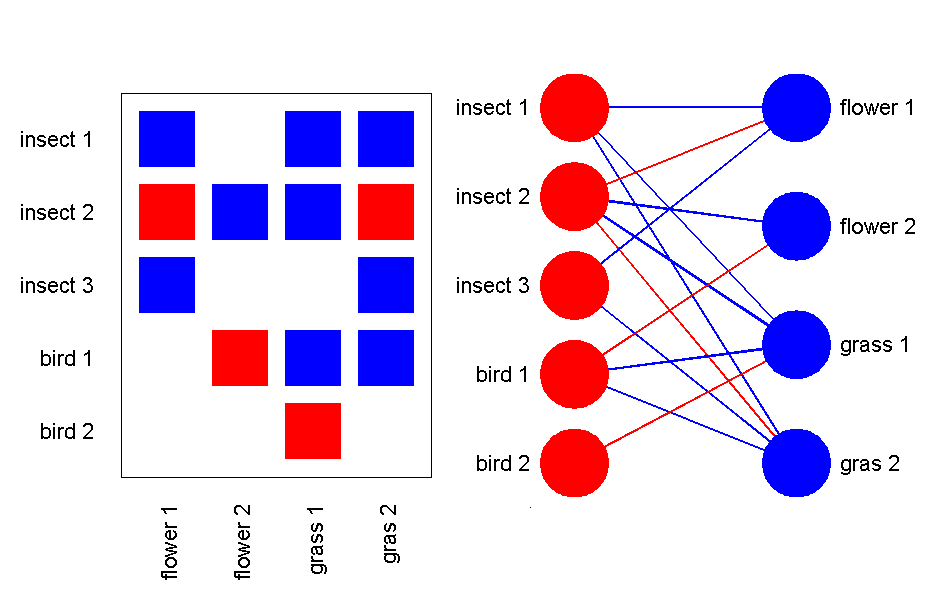
\includegraphics[width=0.6\textwidth]{img/bipartite_class_01.png}
    \caption{A bipartite network in ecology: What animals eat what plants. Source:~\cite{flores2016bimat}}\label{fig:networkecology}
\end{figure}

Usually, when representing bipartite networks, only the edges between the groups
are of interest. However, here we want to infer the weights of the edges
between the groups by also 
looking at the edges within the groups.

We will therefore divide the information of the graph in three matrices. 
There are two matrices that represents the similarity between respectively
the phages or the bacteria, and there is a third matrix that represents the
relation between the phages and the bacteria. Usually a bipartite graph is
only represented using this third matrix, and when referred to the bipartite graph,
this matrix is usually the one that is meant. However, here we will also make use 
of the information of the similarity matrices between phages and between bacteria.

In the relation matrix, or interconnection matrix, 
an edge represents the possibility for a phage to be able to infect the bacterium. 
We will refer to this matrix as $C$. The dimensions of this matrix are
$f \times b$, where $f$ indicates the amount of phages and $b$ indicates the amount
of bacteria. Now, each entry of the matrix represents a relation with one particular
phage and one particular bacteria. 

% In addition to the relation matrix, 
% we have two similarity matrices. One that indicates the similarity of phages
% with other phages. 
The matrix that represents the phage similarity we call $F$ and has dimensions $f \times f$,
where $f$ indicates the 
amount of phages. The other matrix indicates the similarity
of the bacteria with the other bacteria. This matrix we call $B$ and has
dimensions $b \times b$. Unlike the relation matrix $C$, the similarity matrices
are symmetrical. 

\subsection{Modularity and nestedness}

Phage-host relationship graphs are often non-random. They can often be
characterized using measures as modularity and nestedness.

\begin{figure}[hb]
\centering
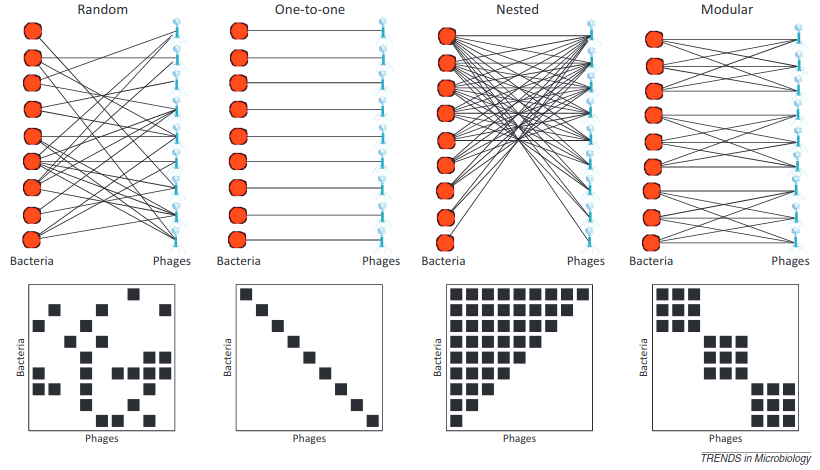
\includegraphics[width=0.55\textwidth]{img/nested_and_modular.png}
\caption{Nested and modular networks. Source:~\cite{weitz2013phage}}
\end{figure}

Modularity in a bipartite graph means that we can define certain
groups that mostly have connections with other nodes in that group, but have fewer
connections with nodes outside the group. Biologically, this probably indicates
that these bacteria and phages are living together and therefore the phages
have mostly evolved to target those specific group of bacteria and cannot
infect other bacteria that are not found in nature with those other phages. 

Nestedness in a bipartite graph means that we can order the graph in such a 
way that there is a hierarchy between phages that target many bacteria 
and phages that only target a few bacteria. For this graph, there are 
general phages, that can target a lot of bacteria, and specialized phages, 
that only target a few. Biologically these patterns are likely caused because
some phages have evolved better attack mechanisms against multiple bacteria,
and some are more lacking behind. Just as some bacteria have evolved better
defense mechanisms than those infected by a lot of phages. 

When investigating published relation matrices of phage-host relationships 
based on empirical data, it is found that these matrices are mostly nested.
However, it is also noted that this observation might be biased by the environments
that have been analyzed in those experiments. Environments like low resource environments,
for example, might eliminate the general phages. Another interesting bias that is discovered,
is that network analysis of microbial communities in food production is often
more modular. These kinds of communities are most likely selected by those food producers
as modular communities are more robust against phage attacks~\cite{weitz2013phage}.

\begin{figure}[htb]
\centering
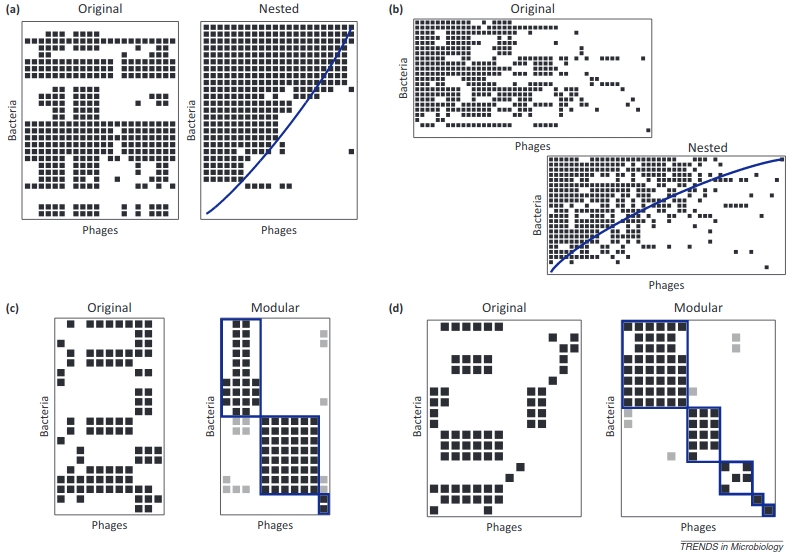
\includegraphics[width=0.8\textwidth]{img/nested-vs-modular.png}
\caption{Nested and modular infection matricies from real data. Source:~\cite{weitz2013phage}}
\end{figure}

\subsection{What data is available}

The proposed method tries to use information that is available for as well
phage-host relationships as well as phage-phage and bacterium-bacterium
relationships / similarities. Sometimes information that is used in the 
similarity calculation can also be used to predict an infection relationship.
Most of these relationships are based on the fact that because phages insert
themselves in the DNA of the bacterium, they will likely have similar DNA, 
or a bacterium might even have traces of the phage found in the bacterium.
Here summarized what these kinds of sources
of information are, found in~\cite{edwards2016computational}.

\subsubsection{Phage-host relationships}

\textbf{Co-abundance in metagenomics} Metagenomic samples are samples from
nature including multiple organisms. Whenever you find a phage and a
bacterium together in the same metagenomic dataset, they live together and
makes it also likely that the phage infects the bacterium.

\textbf{Genetic homology} Since phages integrate their DNA into the bacteria, 
over time some left-overs of genes might still be found in the bacteria. 
Comparing genes in phages and bacteria might give clues about the relationships
the bacteria and phages have.

\textbf{Oligonucleotide profiles} In addition to the genetic homology, you can 
also look on the base pair level itself for relations between different
genomes. In this case, you can look at small pieces of DNA (oligonucleotides or k-mers) 
and match them between organisms.

\textbf{Codon usage} Instead of taking arbitrary k-mers, you can also look 
at the codons and see how much similarity you can find there. In this case
you look at the in frame 3-mers. Codon usage might be important as a phage
needs to make use of the tRNA as the bacterium when infecting.

\textbf{GC content} The least specific way of looking for homology on the
basepair level is to look at the percentage of GC content in the genomes.

\textbf{Exact matches} Since the phages insert themselves in the bacteria, 
it is possible to find complete phages in the bacterium's genome, and thus
confirming a relationship between the found phage and the bacterium.

\textbf{CRISPR} To defend themselves against phages, bacteria have acquired
an immune system that saves the intruders' information in CRISPR arrays. 
Extracting the CRISPR arrays and matching them with phages might give
clues about what phages the bacteria faces.

\subsubsection{Phage-phage relationships}

The metrics uses to match phages and bacteria, can also be used to 
generate the similarity between phages (except CRISPR, and searching for exact matches). 
In addition, you can make use of phylogenetic distances between phages, or look
at the phylogenetic distances of the genes that are used for infiltrating in 
the bacteria.

\subsubsection{Bacterium-bacterium relationships}

Just as for phages, the already mentioned metrics can also be used to find
relationships between bacteria. Even though a CRISPR spacer might not hit
in a phage, using it for bacterium-bacterium similarity can still be helpful
as it still indicates that they (used to) have the same phages that attacked them.
Here we can also focus on the phylogeny
of the proteins of the defense mechanisms of the bacteria.

\subsection{Network fusion}

When creating a network from biological data, a common challenge involves
being able to combine multiple sources of information. This problem is
known as network fusion. 

There are multiple different strategies to solve the network fusion problem. 
Here we propose to make use of an existing method called 
similarity network fusion (SNF)~\cite{wang2014similarity}
with more details here~\cite{wang2012unsupervised}.

For a full explanation of the algorithm,
consult the papers, but in short, you have to create a similarity network
for each source of information and then combine the networks using the 
following algorithm:

First generate a similarity matrix $W$ for each of your information sources, 
then normalize this matrix to create the status matrix.
Take the self-similarity as $\frac{1}{2}$.
Then create a kernel matrix $P$ 
by normalizing using the k-nearest neighbours $N_i$ which 
results in a sparse matrix $P^*$. We will keep using the $*$ to indicate sparseness
by nearest neighbour selection.

\begin{equation}
    P(i, j) = 
    \begin{cases}
        \cfrac{W(i, j)}{2 \sum_{k \neq i}W(i, k)} & j \neq i \\
        \hfil \frac{1}{2} & j = i
    \end{cases}
\end{equation}

\begin{equation} \label{eq:normsparse}
    P^*(i, j) = 
    \begin{cases}
        \cfrac{W(i, j)}{\sum_{i \in N_j}W(i, j)} & i \in N_j \\
        \hfil 0 & else
    \end{cases}
\end{equation} 

Here are the update formulas to fuse the different status matrices $P_v$ and $P_w$ that 
represent two different information sources. Repeat the formulas till convergence.

\begin{align} \label{eq:update}
    \begin{split}
        P_{v, t+1} = P^*_{w, t} \times P_{v, t} \times P^{*,T}_{w, t} \\
        P_{w, t+1} = P^*_{v, t} \times P_{w, t} \times P^{*,T}_{v, t}
    \end{split}
\end{align}

This can be extended to account for more than 2 information sources.

A visualization of this algorithm is depicted in figure~\ref{fig:sim}.

\begin{figure}[ht]
    \centering
    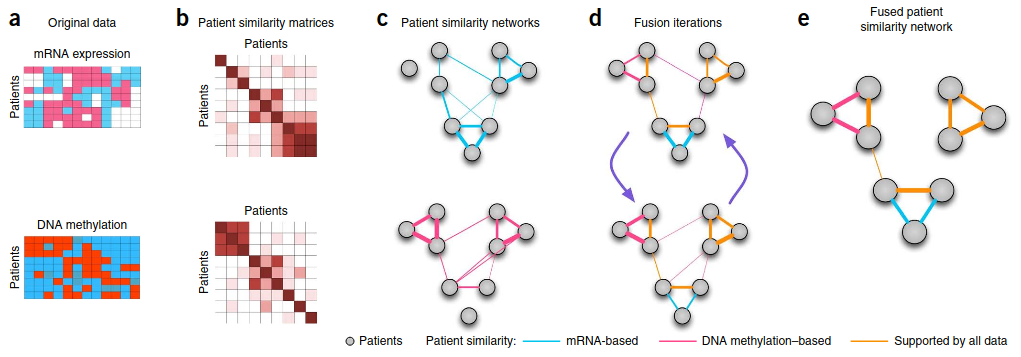
\includegraphics[width=1\textwidth]{img/sim.png}
    \caption{Visualization of SNF. Source~\cite{wang2014similarity}}\label{fig:sim}
\end{figure}

\section{Related work}

As far as I can find, the only computational work done on phage-host relationships 
involves a single metric which is used to measure the possibility of a phage-host relationship~\cite{edwards2016computational}.
I could not find references to an attempt to combine these results or to combine
it with phage-phage or bacterium-bacterium similarity.

For the method conceptually I would find a paper that reports using ``iterative weighted distributed averaging''
to apply network fusion on bipartite graphs~\cite{khan2007distributed}.

\section{Proposed method}

The challenge here is that have different sources of information, 
but we also have two different kinds of similarity matrices, one for bacteria
and one for phages, and we have different sources of information for the third
matrix, the relation matrix. 

The challenge here is that we have three kinds of matrices that all have
different sources of information. We want to combine all this information
and create a single relation matrix.
This proposal shows how all these sources can be
combined to get this relation matrix and using all the different sources of information.
We dot his by proposing modifications of the SNF algorithm useful for bipartite networks.

The assumption we make here, is that related phages target the same bacteria, 
and that related bacteria are target by the same phages. This is most likely
to work best when the bipartite network is also mostly modular, but it will
work as well if the bipartite network is very nested although it could be
that the general phages will diffuse too much or too little to the other phages.

\subsection{Combining different information}

First, the different sources of information for both the phages as the bacteria networks
are combined to present a similarity graph for both the phages and the bacteria.
For this the standard SNF method can be used.

\subsection{Diffusion of the phage-host relationship}

Now we have a similarity network for both the phages as the bacteria. 
The next step will be to `diffuse' the information that exist for phage-host 
relationships (the connection graph) 
to other phage-host connection that don't have this information
available.  
We diffuse the weights to other connections that have the most similar phages
or the bacteria. This idea is worked graphically depicted in figure~\ref{fig:phagediff}.

To do this we first pick what network to use (either the phage-phage $F$, or 
the bacterium-bacterium $B$). (It is probably best to make use of the sparse
similarity matrix here, $F^*$ and $B^*$.).
Then multiply this with the connection matrix ($C$). This will then move the
weights over the strongest connection for each phage or bacterium.

When working out the math it will become clear that the steps for the phage
similarity matrix and the bacteria similarity matrix can be combined into 
a single step that has much resemblance to the previous discussed SNF algorithm. 

\begin{minipage}{\textwidth}
Here we find the update rule to move from $C_{t-1}$ to $C_{t}$ to $C_{t+1}$ in 
one step. These steps can be repeated $n$ times.

\begin{align}
    \begin{split}
    C_{t+1} &= F^* \times C_t \\
    C_{t} &= (B^* \times C_{t - 1}^{T})^{T} \\
          &= C_{t - 1} \times B^{*,T} \\
    \hfil Combined: \\
    C_{t+1} &= F^* \times C_{t - 1} \times B^{*,T}
    \end{split}
\end{align}

\end{minipage}

\hfill

\begin{figure}[hb]
    \centering
    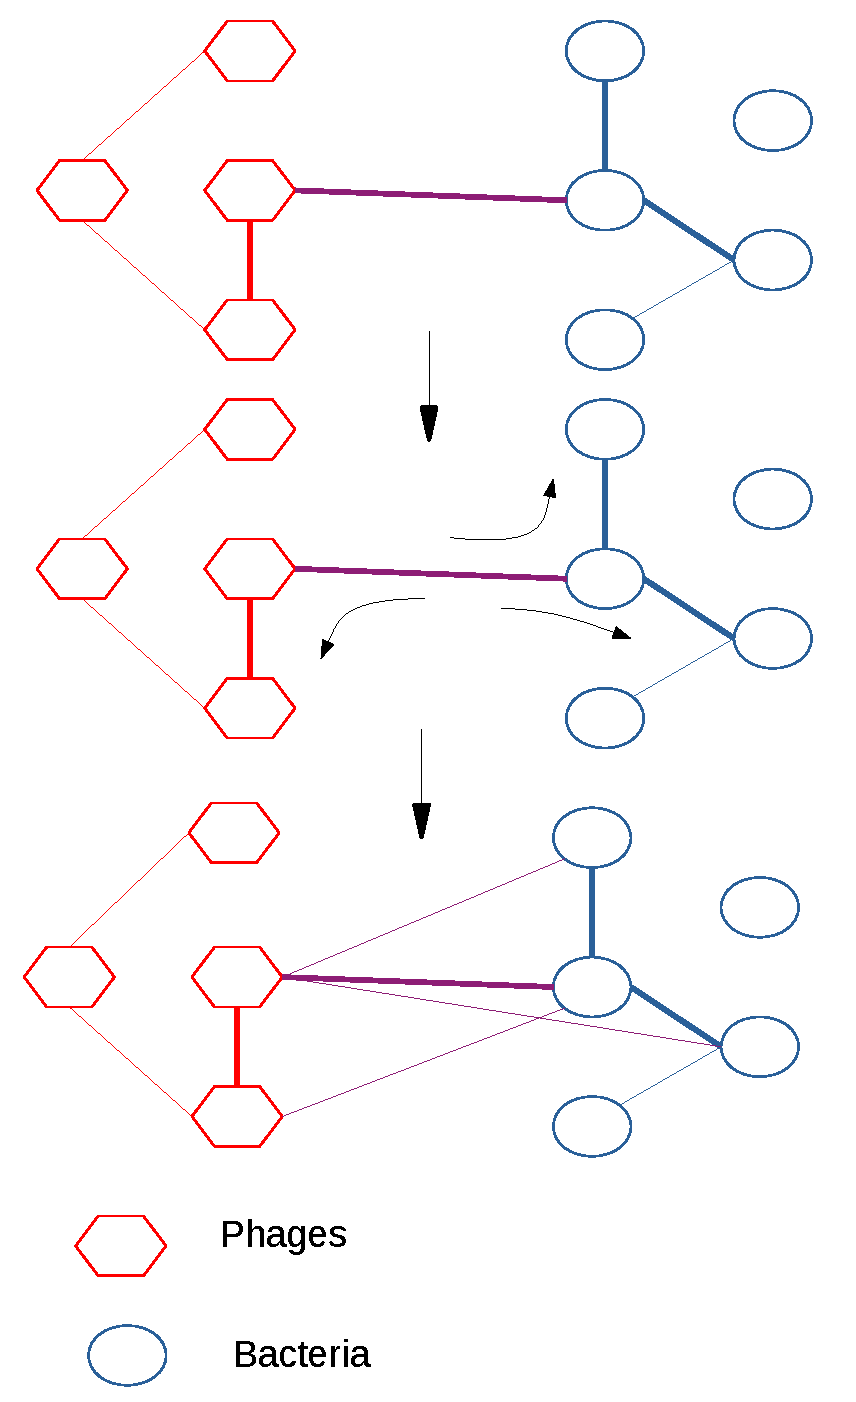
\includegraphics[width=0.5\textwidth]{img/phage-bac-diffusion_cropped.pdf}
    \caption{Visualization of diffusion of relation matrix (purple) using the similarity matrices (red for phages, and blue for bacteria).}\label{fig:phagediff}
\end{figure}

\subsubsection{Modification to ensure convergence}

Since we are alternating between two different similarity matrices,
I think it will not converge.
To make sure the algorithm converges, I propose to modify the
similarity matrices every iteration by gradually reducing the percentage of weight
that gets moved around until it reaches zero percent.

This can be mathematically be accomplished by changing the normalization
function of formula~\ref{eq:normsparse}.
Let the self-similarity start at some point ($a(0) = \frac{1}{2}$) 
and let it gradually grow to one. 
When it reaches one, the normalization transforms the similarity matrix into
an identity matrix. Now all similarity is self-similarity 
and no weight is shifted anymore. 
Multiplication with an identity matrix does not change the matrix anymore.
Keep in mind that this change of normalization only happens for the 
similarity matrices. The relation matrix remains untouched by the transformation, 
and will gradually change less and less until the similarity matrices transforms
into a identity matrix. 

\begin{equation}
    \begin{gathered}
    P^*(i, j) = 
    \begin{cases}
        (1 - a(t)) \times \cfrac{W(i, j)}{\sum_{i \in N_j}W(i, j)} & i \in N_j \\
        \hfil a(t) & i = j \\
        \hfil 0 & else
    \end{cases} \\
    a(0) = \frac{1}{2} \\
    a(T) = 1
    \end{gathered}
\end{equation}

What's more, this adjustment can help to prevent weights drift too far away and
can thereby preserve some nestedness. It is therefore probably also best
that this function that is responsible for reducing the amount of shifted weight
is convex so that most of the change happens in the 
first iteration. I believe this will be best to prevent disrupting the 
nestedness too much, but it can be experimented with what would be best.

\subsubsection{Performing network fusion on the connection matrix}

Now we only are left with multiple connection matrices for each source of 
information on the phage-host relationships. We can however transform the
connection matrix in a square matrix ($M$) by adding the missing edges between
bacteria and phages as an edge with zero. So, in essence we stack
the connection matrix with the similarity matrix of the phages and the bacteria.
The resulting matrices can then
be fused using the aforementioned SNF fusion algorithm. This can in fact
be simplified by applying similar to the SNF fusion algorithm to the connection matrix 
directly. 

Here we merge connection matrix $C_w$ with $C_v$. In the derivation $0_x$ indicates a square with all zeros with size x by x.

\begin{equation}
\begin{gathered}
    \textit{Full matrix from connection matrix:} \\
    M = \begin{bmatrix}
            0 & C^T \\
            C & 0
        \end{bmatrix} 
\end{gathered}
\end{equation}
\begin{equation}
\begin{gathered}
    \textit{Update rules (see formula~\ref{eq:update}):} \\
    M_{v, t+1} = M^*_{w, t} \times M_{v, t} \times M^{*,T}_{w, t} \\
    M_{w, t+1} = M^*_{v, t} \times M_{w, t} \times M^{*,T}_{v, t}
\end{gathered}
\end{equation}
\begin{equation}
\begin{aligned}
    M_{v, t+1} &= M^*_{w, t} \times M_{v, t} \times M^{*,T}_{w, t} \\
               &= \begin{bmatrix}
                   0_b & C^{*,T}_w \\
                   C^*_w & 0_f
               \end{bmatrix} \times 
               \begin{bmatrix}
                   0_b & C^T_v \\
                   C_v & 0_f
               \end{bmatrix} \times
               \begin{bmatrix} 
                   0_b & C^{*,T}_w \\
                   C^*_w & 0_f
               \end{bmatrix} \\
               &= \begin{bmatrix}
                   0_b & C^{*,T}_w C_v C^{*,T}_w \\
                   C^*_w C^T_v C^*_w & 0_f
                   \end{bmatrix} \\
     C_{v,t+1} &= C^{*,T}_w C_v C^{*,T}_w
\end{aligned}
\end{equation}

\begin{figure}[hb]
    \centering
    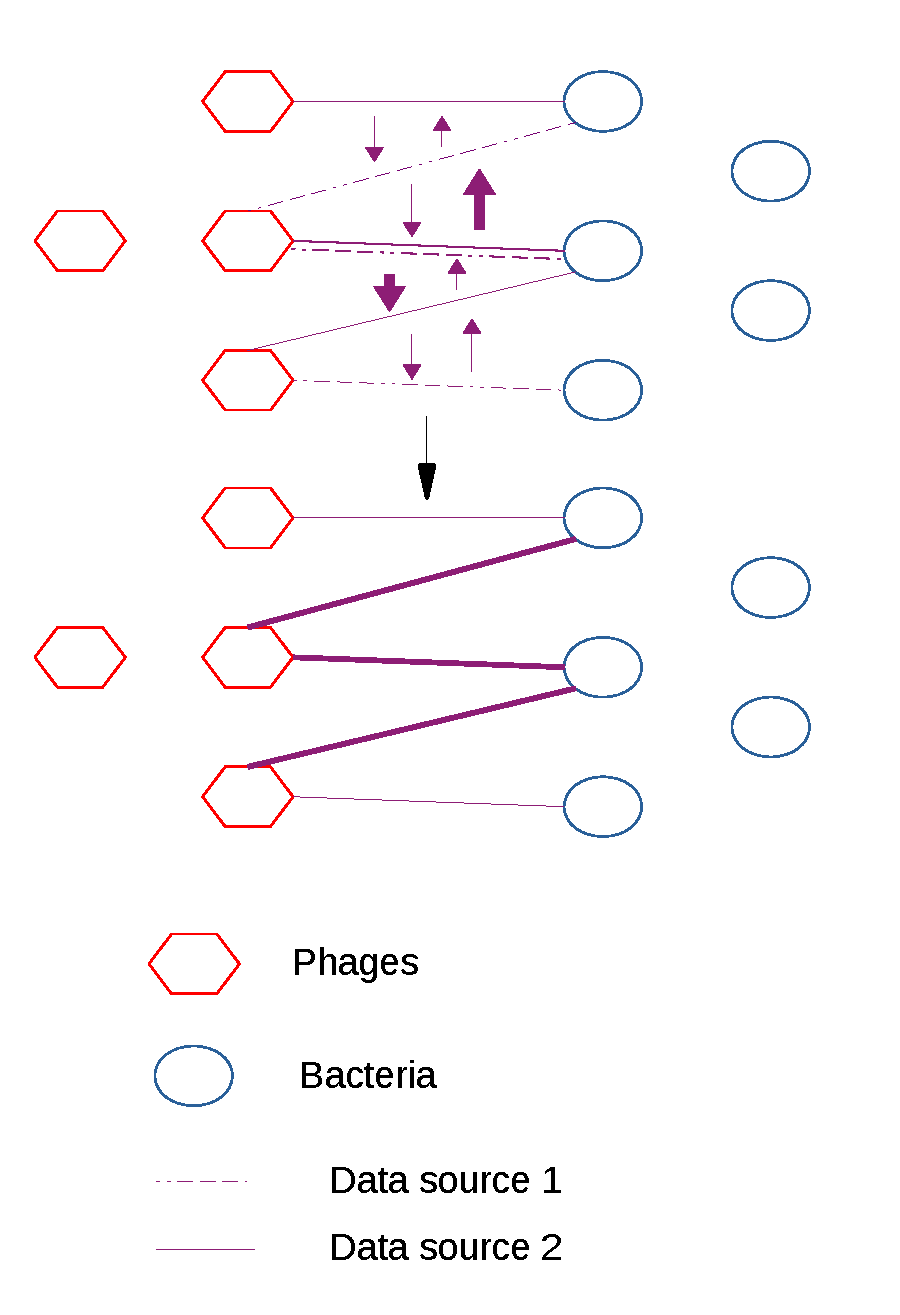
\includegraphics[width=0.6\textwidth]{img/connection-diff_cropped.pdf}
    \caption{Visualization of the diffusion of the connection matrix.}\label{fig:connectdiff}
\end{figure}

\subsubsection{Discussion: A note on the order and combination of steps}

As can be seen, there are a few different ways to combine all the information.
You can for example also apply the network fusion on the connection matrix
first and then diffuse it using the similarity matrices. This is also 
faster because then the diffusion is only applied to one connection matrix
and not multiple. I think this might be a worthwhile alternative to investigate.

On the other hand, you can even apply the diffusion
using the different sources of the similarity matrices. I, however, don't
think that is the best way as it then will start to mix different kinds 
of information too much too early. Although, you can also argue that information
might be lost too soon, so this is probably is something that needs to be
experimented with a bit.

Finally, you can
also create the full square matrix from the connection matrix by including the
similarity weights already instead of setting those edges to zero. I also 
think that such an approach tries to combine too much information too early.
However, it might still be interesting to investigate the affect between
forcefully setting the similarities between bacteria and phages to zero 
or to let them grow as well, or even initialize them to some value (fixed
or otherwise). Setting those to the identity matrix of a fraction of that 
is also another option.

\subsubsection{A note on computational complexity}

To reduce the computational complexity, I propose to make the similarity matrices sparse by only
looking at the k-nearest neighbours for each similarity neighbour.
This is also done in the SNF algorithm and can also trivially be applied 
to the aforementioned formulas, and have been indicated using $*$.
Even if the size of the dataset is not that big that reducing the
computational complexity is required, taking the sparse matrix might 
result in better accuracy as it reduces noise for the furthest away neighbors.

\subsubsection{Notes on modular versus nestedness}

The approach relies on the assumption that phage-host networks are
modular. Best case scenario would be in situations where one wants to place
unknown bacteria or phages in a spot with already fairly known relationship. 

However, good results should also be achieved for relative nested networks,
but only if it is 
true that generalized phages and general bacteria are relatively very 
similar to a lot of other respectively phages and 
the specialized phages / less targeted bacteria are more unique. 

\section{Summary}

The discussed method can be summarized in four steps (not necessarily in this order):

\begin{itemize}
\item Find similarity matrices for phage-phage and bacterium-bacterium using network fusion.
\item Find connection matrix for phage-host.
\item Diffuse the phage-host matrix using the phage-phage and bacterium-bacterium matrix.
\item Apply network fusion to the resulting diffused phage-host relationships.
\end{itemize}

\section{Further ideas}

\subsection{Maximizing modularity}

Although modularity is not an end in itself, a modular network is
something what can be expected in some extent.
That's why it might be worth looking into methods 
that focus on maximizing
the weights on the different information sources so that modularity arises,
instead of applying the network fusion algorithm.
This can be done on the connection matrix alone 
(and so still have the ability to perform network fusion and diffusion first),
but can also be done on the combined matrix with 
all the phage-phage and bacterium-bacterium information already included.  
This might however, force a modular network a bit too much.

Additionally, it might be that certain changes to some update formulas can
force a certain degree of modularity. One can see if this is possible and
improves the results.

\subsection{Using experimentally proven phage-host relationships}

There is various experimentally proven phage-host relationships available. 
These experimental data can be used to enhance the network fusion or 
to validate our method. 

Still, it is important to note that those experimentally reported phage-host
relationships might be biased and using it needs caution.

\subsubsection{Enhancing the proposal with some semi-supervised method}

It might be possible to use this as an alternative information source that
can make certain relationships more important than others because
of it being experimentally proven, or can be used in some other semi-supervised
learning way.

\subsubsection{Validation}

This source of information can however also be used a way to validate
our method. 

It is perhaps also a good idea to see if certain assumptions we make in 
this proposal are true for the real world. 
Especially the idea that phages that infect the same
bacteria are more similar to each other and bacteria with the same phages
as viruses are more similar to each other.

\printbibliography{}

\end{document}
